\chapter{Experiment}
\label{c:exp}

\section{Atomic force microscopy}

\begin{figure}[htb]
\centering
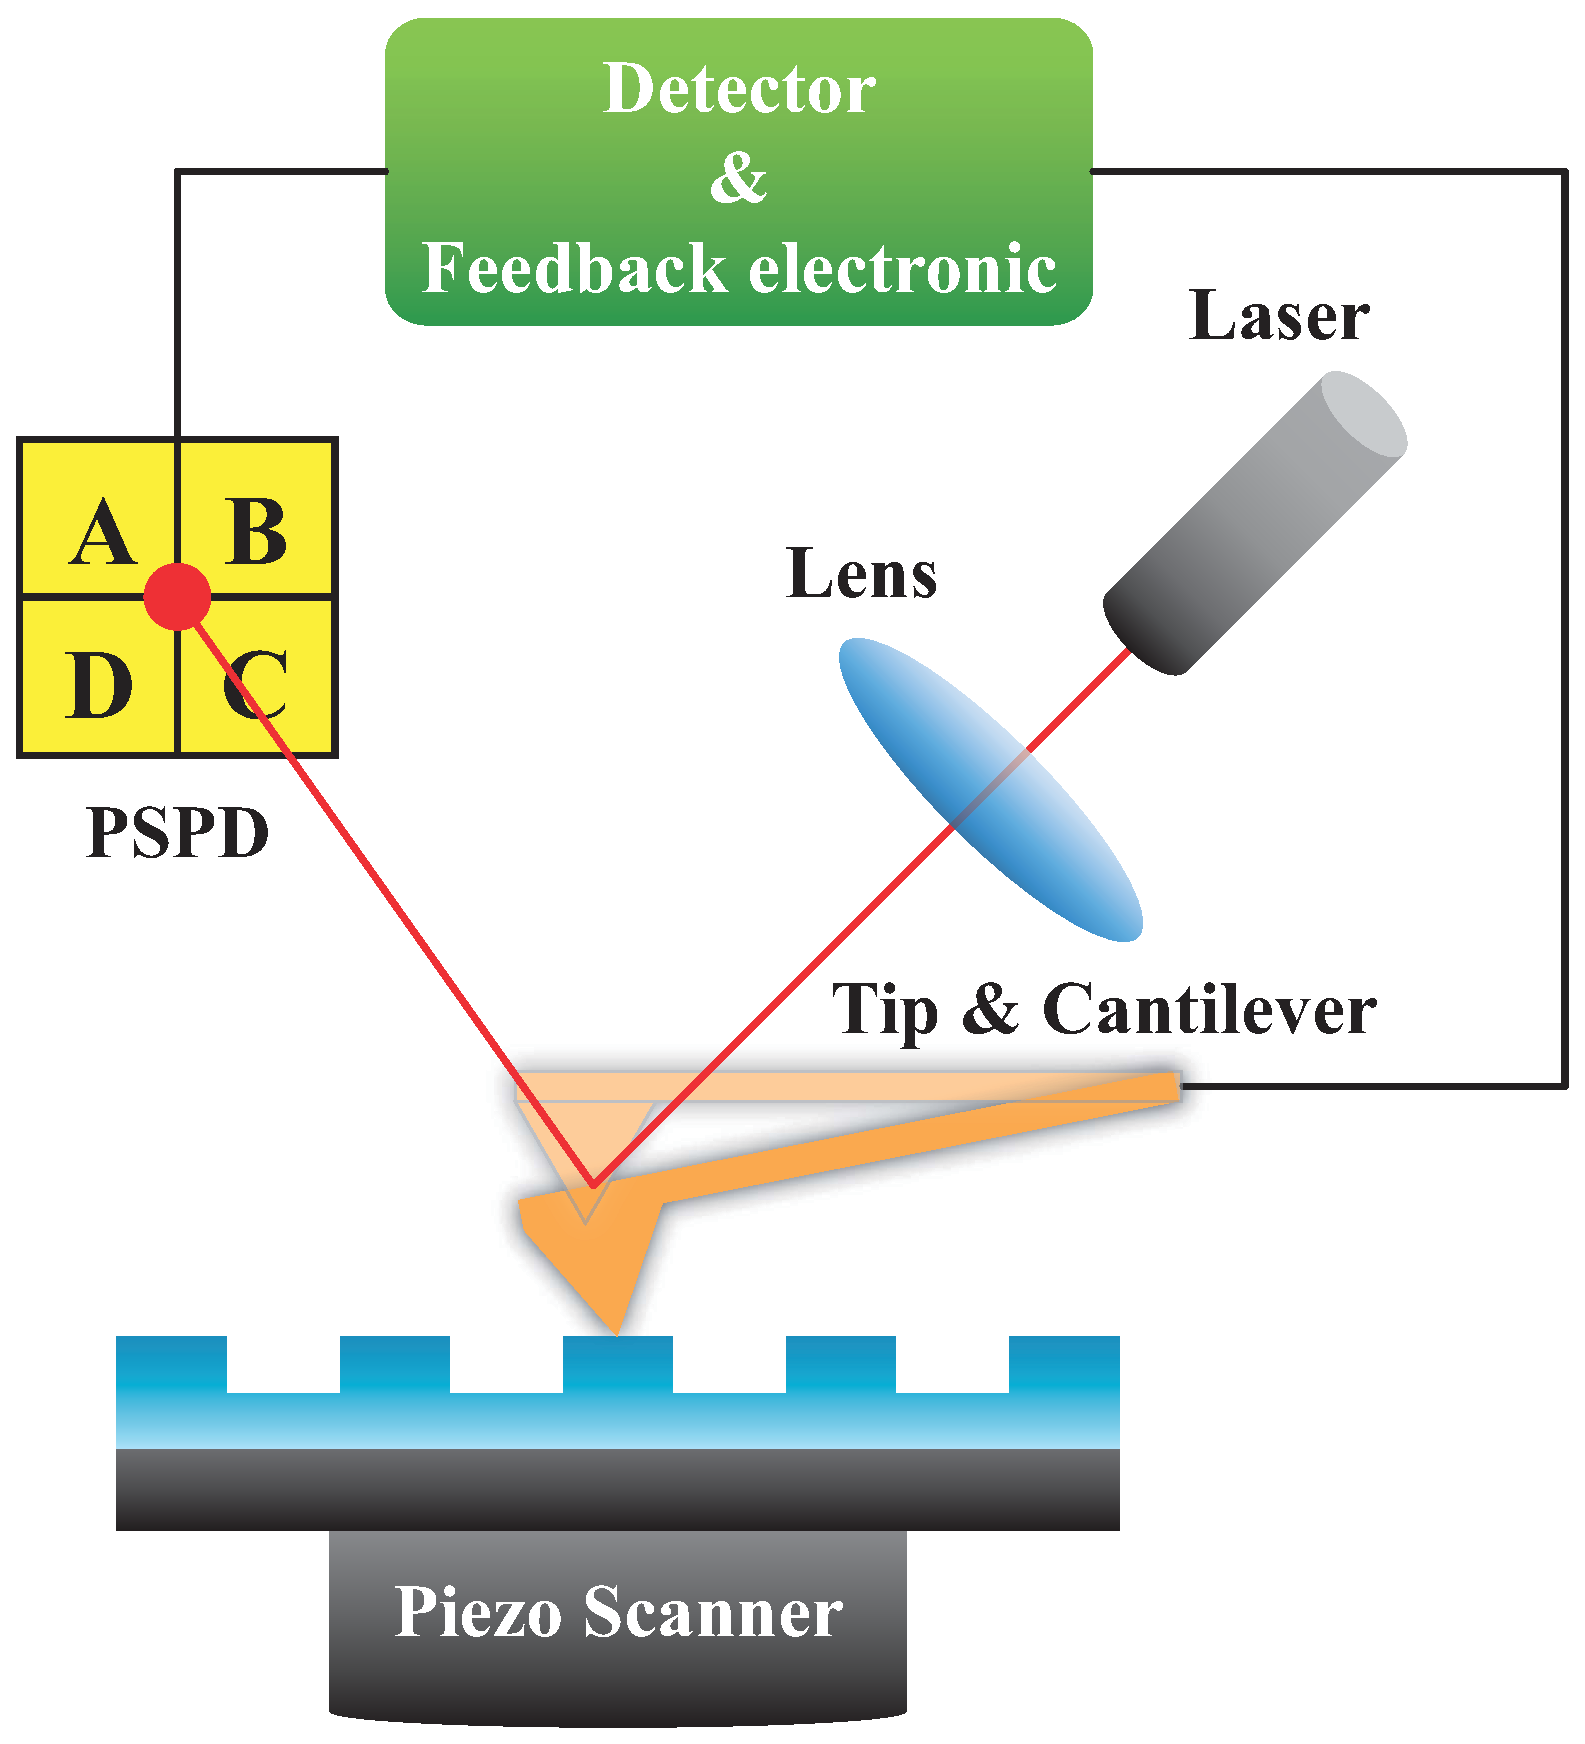
\includegraphics[scale=0.35]{EXP/afm1.eps}
\caption{\label{fig:afm1}Schematic of atomic force microscopy.}
\end{figure}
Atomic force microscope (AFM) is a type of scanning probe microscopes (SPM)~\cite{bennig1988atomic}.  The schematic of AFM is shown in Figure~\ref{fig:afm1}. AFM operates by measuring force between a probe and the specimen surfaces. In general,  the probe is a sharp tip at a cantilever's end. The cantilever can be deflected by atomic forces to sufficiently large amount, then AFM can measure the vertical and lateral deflections of the cantilever by using the optical system. A laser beam is transmitted to cantilever, and the reflected laser beam is detected with a position-sensitive photo detector (PSPD). PSPD is four-sectional that allows measuring not only vertical but lateral bending too(Figure~\ref{fig:afm2}). The output of the PSPD is provided to a computer for processing of the data for providing a topographical image of the surface with atomic resolution, and controlling the height between probe and specimen surfaces by applying voltage on piezoelectric scanner.
\begin{figure}[htb]
\centering
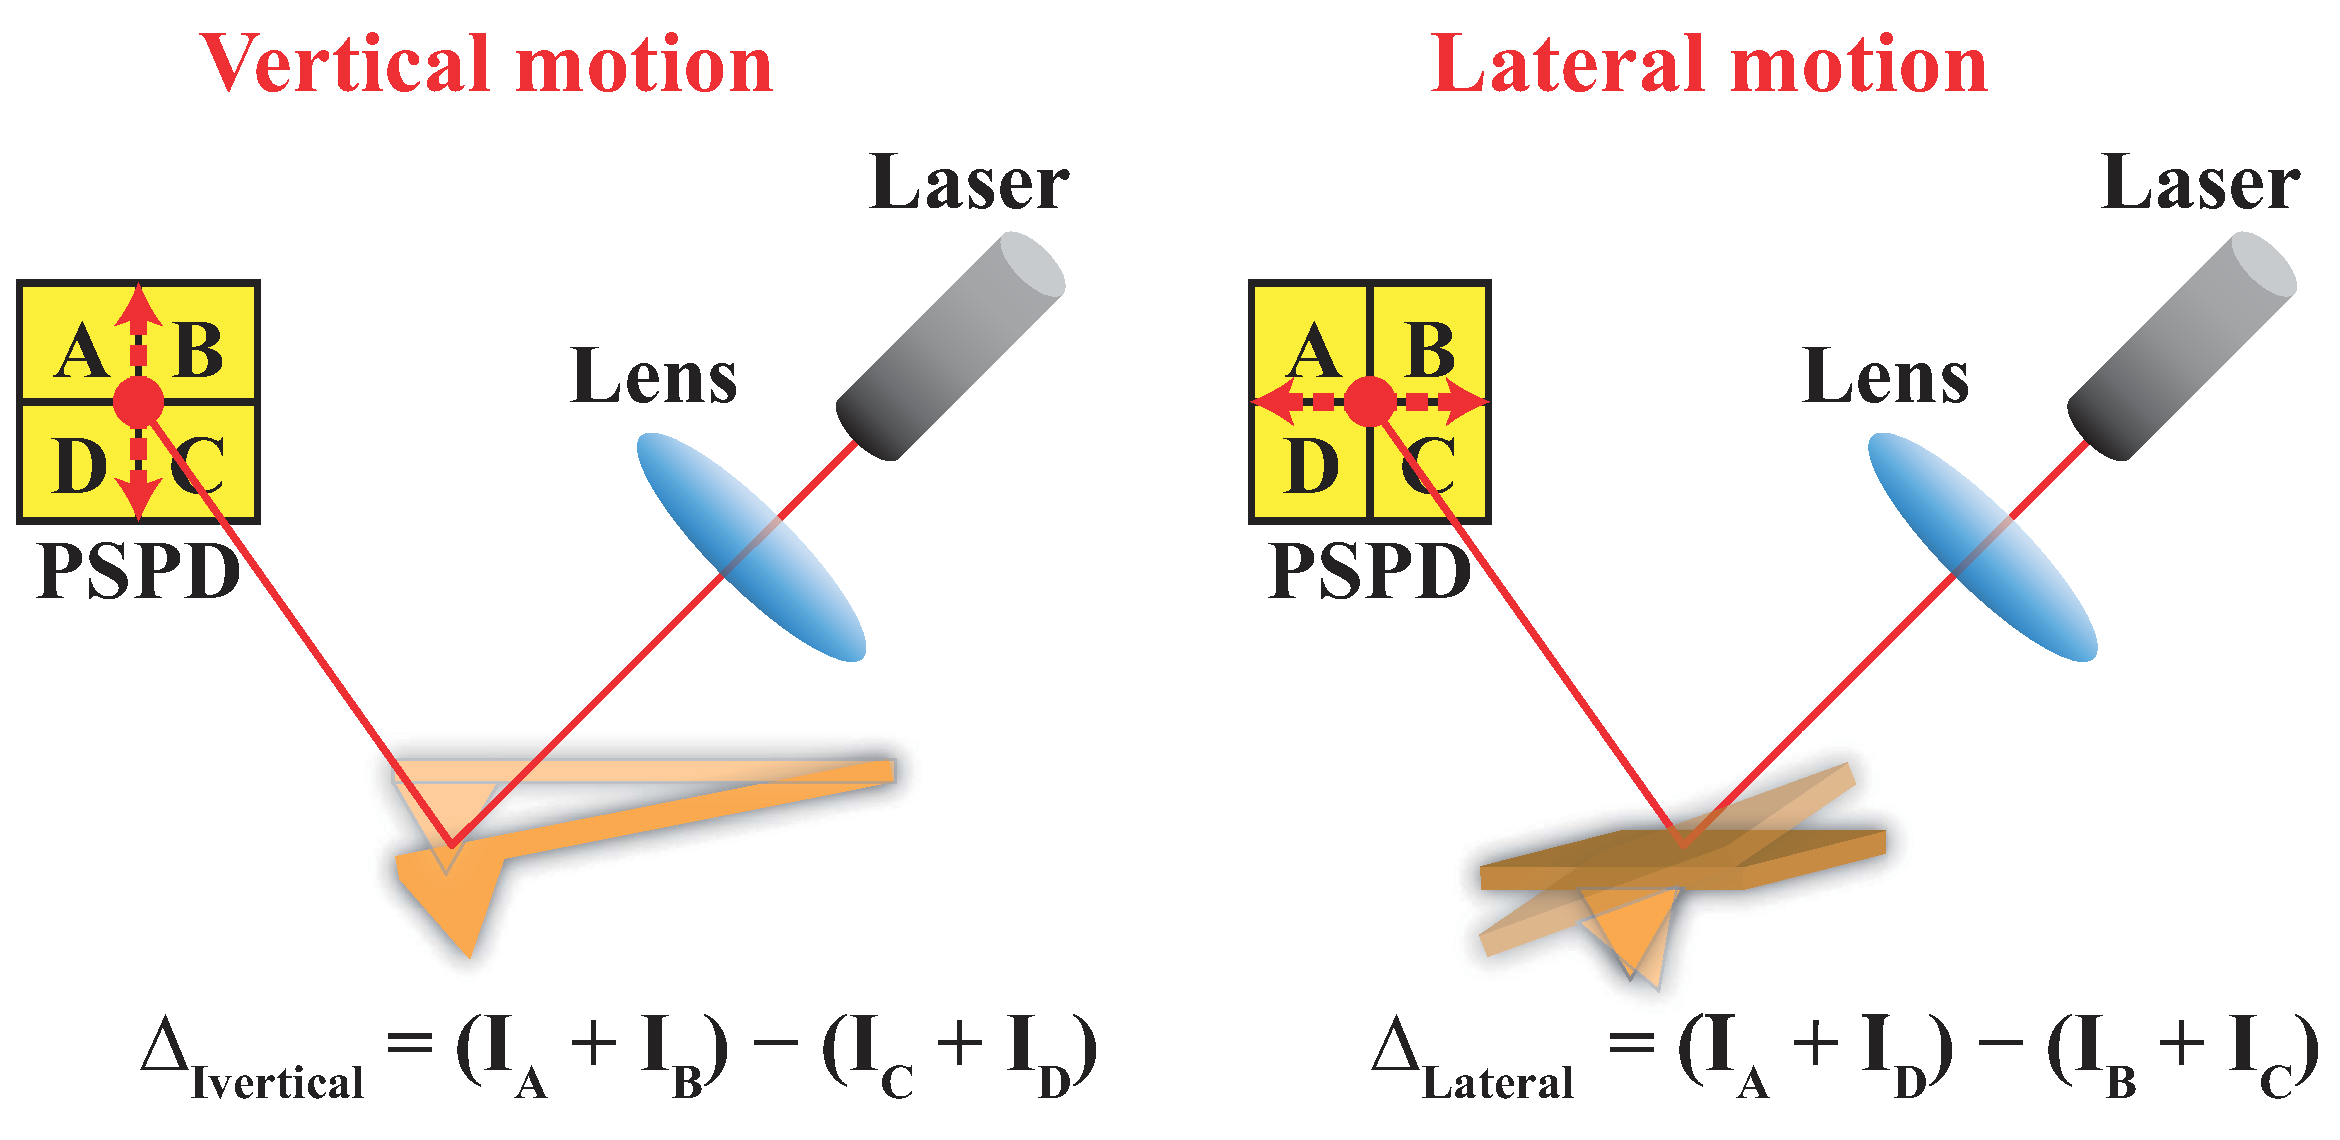
\includegraphics[scale=0.4]{EXP/afm2.eps}
\caption{\label{fig:afm2}Schematic of optical system for cantilever deflections detection.}
\end{figure}

The physical principle of the AFM operation is based on interaction between the probe tip and the specimen surface(Figure~\ref{fig:afm3}). When the cantilever approaches the specimen surface, Van der Waals forces start acting upon it . They are sufficiently far-ranging and are felt at the distance of a few tens of angstroms. Then at the distance of several angstroms repulsive force starts acting. In humid air a water layer is present on the specimen surface. The capillary force arises that holds the tip in contact with the surface and increases the minimum achievable interaction force. Electrostatic interaction between the probe and the sample may appear rather often. This can be both attraction and repulsion. Van der Waals attraction forces, capillary, electrostatic and repulsion forces at the point where the tip touches the sample and forces acting upon the tip from the deformed cantilever compensate each other in equilibrium. Based on the type and degree of this interaction the AFM modes can be broken down into contact and semi-contact(Figure~\ref{fig:afm3} ), which is a transition mode between the contact and non-contact modes.
\begin{figure}[htb]
\centering
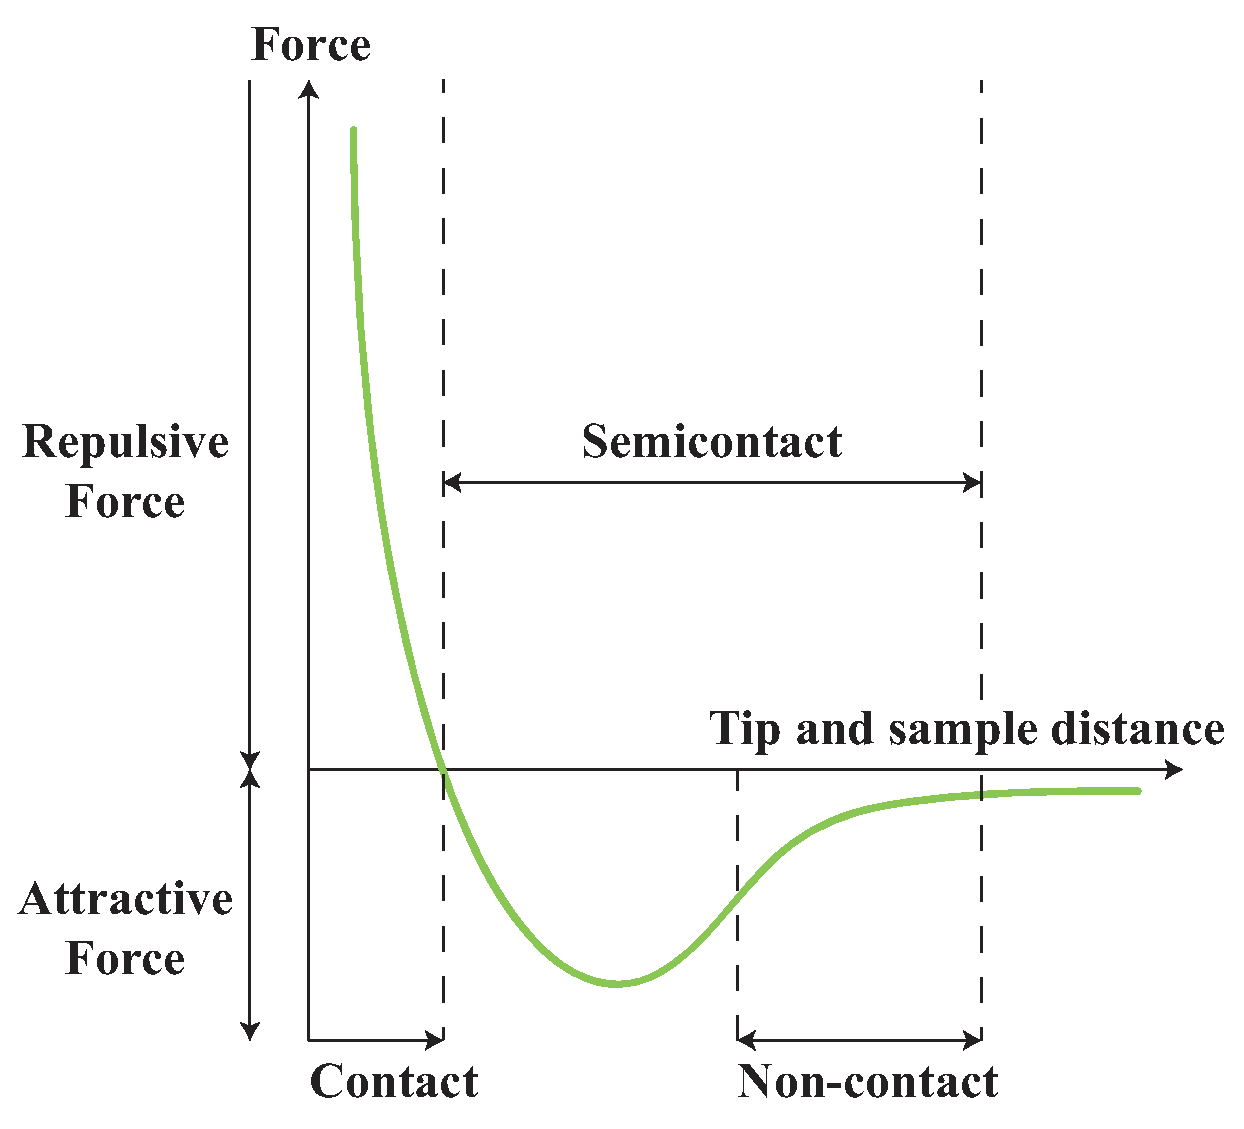
\includegraphics[scale=0.6]{EXP/afm3.eps}
\caption{\label{fig:afm3}Sketch of tip-sample forces.}
\end{figure}

\paragraph{Contact mode}

In contact mode of operation the cantilever deflection under scanning reflects repulsive force acting upon the tip. Repulsion force $\mathbf{F}$ acting upon the tip is related to the cantilever deflection value $\mathbf{x}$ under Hooke's law: $\mathbf{F}=-K \cdot  \mathbf{x}$, where $K$ is cantilever spring constant. The spring constant values for different cantilevers usually vary from 0.01 to several $\mathbf{N/m}$.

In our units the vertical cantilever deflection value is measured by means of the optical registration system and converted into electrical signal DFL (difference signal between the upper and lower halves of the PSPD) . In contact mode the DFL signal is used as a parameter characterizing the interaction force between the tip and the surface. There is a linear relationship between the DFL value and the force. In constant force mode of operation the deflection of the cantilever is maintained by the feedback circuitry on the preset value. So vertical displacement of the scanner under scanning reflects topography of sample under investigation.

Contact force microscopy is surface topography measurement in the contact mode.The microscope operation in the mode of maintaining constant interaction force between the tip and the surface sample, and is the base for measuring surface topography as well as for measuring local rigidity, local viscosity and local friction force. Constant force mode has some advantages and disadvantages. Main advantage of constant force mode is possible to measure with high resolution simultaneously with topography and some other characteristics, such as friction forces, spreading resistance etc. Constant force mode has also some disadvantages. Speed of scanning is restricted by the response time of feedback system. When exploring soft samples they can be destroyed by the scratching because the probe scanning tip is in direct contact with the surface. Therefore, under scanning soft unhomogeneous samples the local flexure of sample surface varies. As a result acquired topography of the sample can be proved distorted. Possible existence of substantial capillary forces imposed by a liquid adsorption layer can decrease the resolution.

\paragraph{Semi-contact mode}

The semi-contac mode can be characterized by some advantages in comparison with contact mode. First of all, in this mode the force of pressure of the cantilever onto the surface is less, that allows to work with softer materials such as polymers and bio-organics. The semi contact mode is also more sensitive to the interaction with the surface that gives a possibility to investigate some characteristics of the surface distribution of magnetic and electric domains, elasticity and viscosity of the surface. 

Widely used semi-contact mode has some disadvantage concerned with the usage of the feedback circuit. The scanning speed in semi-contact mode is restricted by the feedback circuit reaction time. This disadvantage can be overcome by the fact that under scanning new value of cantilever oscillation amplitude (and error signal) usually is achieved faster than preset value of the cantilever oscillation amplitude can be reached by the feedback system. Time of the reaching new value of the oscillation amplitude is determined by the oscillation period and Q-quality of the cantilever.
The feedback error signal, emerging when scanning in the semi-contact mode, contains some additional information about the topography. It can be utilized for achieving a more precise recovery of the relief. 

Additionally, similarly to the contact error mode, which can be considered as intermediate between the constant force mode and constant height mode, the feedback gain factor (i.e. the feedback processing speed) can be adjusted for the system to be able to trace subtle changes of the relief and to be too slow to trace the steep changes. Then, when the probe travels over minor irregularities, scanning will be carried out with an almost constant piezo scanner length. As a result, the slow changes of the relief will hardly show up on the images, and the steep changes will appear in high contrast. This may be helpful in finding minor irregularities on large areas against major sloping relief features. It must be noted that height of the minor irregularities must be less than amplitude of cantilever oscillation.

\section{Scanning electron microscopy}

The scanning electron microscope (SEM) is used for the observation of specimen surfaces~\cite{von1938elektronen}. When the specimen is irradiated with a fine electron beam, secondary electrons are emitted from the specimen surface. Topography of the surface can be observed by two-dimensional scanning of the electron probe over the surface and acquisition of an image from the detected secondary electrons. The concept schematic of commercial SEM (JEOL, JSM-6500F) is shown in Figure~\ref{fig:sem1}. The basic unit is composed of an electron optical system, a specimen stage, a secondary-electron detector, an image display unit, and an operation system. The electron optical system consists of an electron gun, a condenser lens and an objective lens to produce an electron probe, a scanning coil to scan the electron probe, and other components. The system inside of the microscope column are kept at vacuum.
\begin{figure}[htb]
\centering
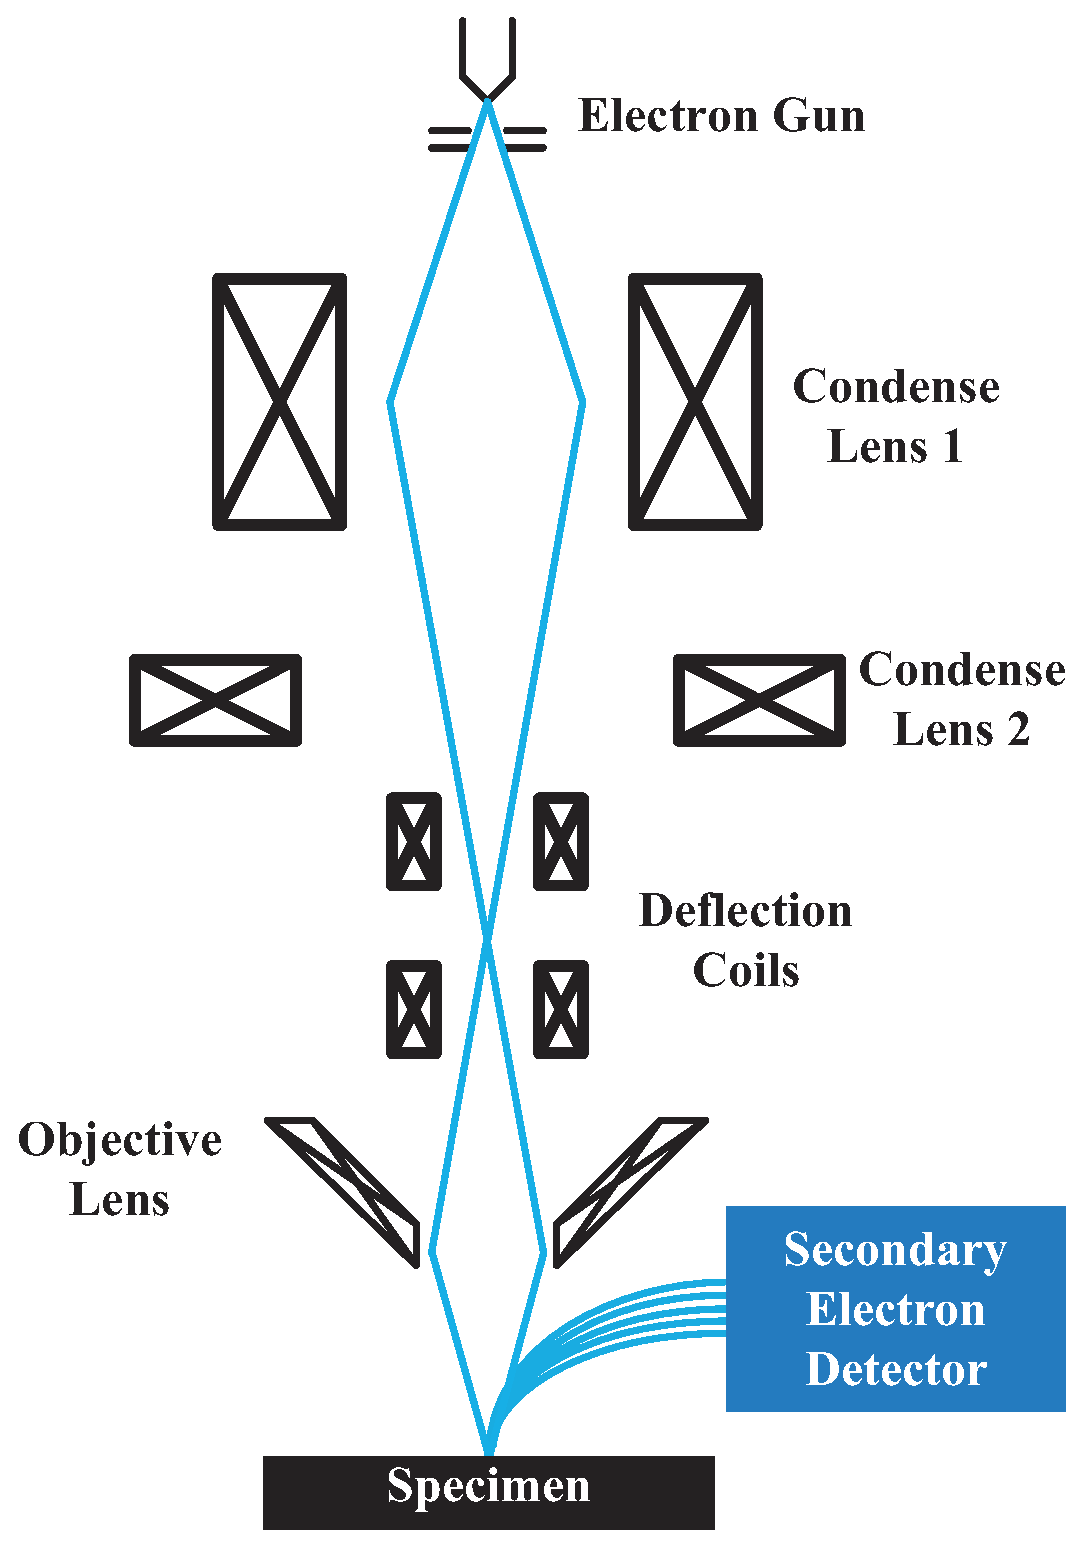
\includegraphics[scale=0.5]{EXP/SEM.eps}
\caption{\label{fig:sem1}Basic construction of a scanning electron microscopy.}
\end{figure}


The JSM-6500F utilizes a Schottky type field-emission (T-FE) gun for the electron source. The T-FE gun can constantly supply the surface of the cathode with zirconium oxide by heating the surface of cathode to 1800 K. For this reason, it can easily obtain stable and high probe current (range from several pA to 100 nA) compared with the traditional thermal emission electron gun and cold field-emission gun.

The magnetic condenser and objective lens system act to control the diameter of the beam as well as to focus the beam on the specimen due to a rotationally-symmetric magnetic field is formed when we pass a direct electric current through a coilwound electric wire in the magnetic lens. A pair of deflector coils, which between the condenser and objective lens, controlled by the scan generator, which are responsible for rastering that focused beam across the specimen surface. The size of the rastering pattern is under magnification control. The beam is rastered from left to right and top to bottom. There is a one-to-one correspondence between the rastering pattern on the specimen and the rastering pattern used to produce the image on the monitor. The resolution we choose to image at will obviously affect the number of pixels per row as well as the number of rows that constitute the scanned area.

The signal is generated from the specimen, and collected by the detector and subsequently processed to generate the image. That processing takes the intensity of the signal coming from a pixel on the specimen and converts it to a grayscale value of the corresponding monitor pixel. The monitor image is a two dimensional rastered pattern of grayscale values.

With the beam focused on the specimen surface, all we need to do to change magnification is to change the size of the rastered area on the specimen. The size of the monitor raster pattern is constant. Magnification will increase if we reduce the size of the area scanned on the specimen.

%\bibliographystyle{unsrt}
%\bibliography{thesisbib}